\documentclass[]{article}
\usepackage{lmodern}
\usepackage{amssymb,amsmath}
\usepackage{ifxetex,ifluatex}
\usepackage{fixltx2e} % provides \textsubscript
\ifnum 0\ifxetex 1\fi\ifluatex 1\fi=0 % if pdftex
  \usepackage[T1]{fontenc}
  \usepackage[utf8]{inputenc}
\else % if luatex or xelatex
  \ifxetex
    \usepackage{mathspec}
    \usepackage{xltxtra,xunicode}
  \else
    \usepackage{fontspec}
  \fi
  \defaultfontfeatures{Mapping=tex-text,Scale=MatchLowercase}
  \newcommand{\euro}{€}
\fi
% use upquote if available, for straight quotes in verbatim environments
\IfFileExists{upquote.sty}{\usepackage{upquote}}{}
% use microtype if available
\IfFileExists{microtype.sty}{%
\usepackage{microtype}
\UseMicrotypeSet[protrusion]{basicmath} % disable protrusion for tt fonts
}{}
\usepackage[margin=1in]{geometry}
\usepackage{color}
\usepackage{fancyvrb}
\newcommand{\VerbBar}{|}
\newcommand{\VERB}{\Verb[commandchars=\\\{\}]}
\DefineVerbatimEnvironment{Highlighting}{Verbatim}{commandchars=\\\{\}}
% Add ',fontsize=\small' for more characters per line
\usepackage{framed}
\definecolor{shadecolor}{RGB}{248,248,248}
\newenvironment{Shaded}{\begin{snugshade}}{\end{snugshade}}
\newcommand{\KeywordTok}[1]{\textcolor[rgb]{0.13,0.29,0.53}{\textbf{{#1}}}}
\newcommand{\DataTypeTok}[1]{\textcolor[rgb]{0.13,0.29,0.53}{{#1}}}
\newcommand{\DecValTok}[1]{\textcolor[rgb]{0.00,0.00,0.81}{{#1}}}
\newcommand{\BaseNTok}[1]{\textcolor[rgb]{0.00,0.00,0.81}{{#1}}}
\newcommand{\FloatTok}[1]{\textcolor[rgb]{0.00,0.00,0.81}{{#1}}}
\newcommand{\CharTok}[1]{\textcolor[rgb]{0.31,0.60,0.02}{{#1}}}
\newcommand{\StringTok}[1]{\textcolor[rgb]{0.31,0.60,0.02}{{#1}}}
\newcommand{\CommentTok}[1]{\textcolor[rgb]{0.56,0.35,0.01}{\textit{{#1}}}}
\newcommand{\OtherTok}[1]{\textcolor[rgb]{0.56,0.35,0.01}{{#1}}}
\newcommand{\AlertTok}[1]{\textcolor[rgb]{0.94,0.16,0.16}{{#1}}}
\newcommand{\FunctionTok}[1]{\textcolor[rgb]{0.00,0.00,0.00}{{#1}}}
\newcommand{\RegionMarkerTok}[1]{{#1}}
\newcommand{\ErrorTok}[1]{\textbf{{#1}}}
\newcommand{\NormalTok}[1]{{#1}}
\usepackage{graphicx}
\makeatletter
\def\maxwidth{\ifdim\Gin@nat@width>\linewidth\linewidth\else\Gin@nat@width\fi}
\def\maxheight{\ifdim\Gin@nat@height>\textheight\textheight\else\Gin@nat@height\fi}
\makeatother
% Scale images if necessary, so that they will not overflow the page
% margins by default, and it is still possible to overwrite the defaults
% using explicit options in \includegraphics[width, height, ...]{}
\setkeys{Gin}{width=\maxwidth,height=\maxheight,keepaspectratio}
\ifxetex
  \usepackage[setpagesize=false, % page size defined by xetex
              unicode=false, % unicode breaks when used with xetex
              xetex]{hyperref}
\else
  \usepackage[unicode=true]{hyperref}
\fi
\hypersetup{breaklinks=true,
            bookmarks=true,
            pdfauthor={Diego Aviles},
            pdftitle={test},
            colorlinks=true,
            citecolor=blue,
            urlcolor=blue,
            linkcolor=magenta,
            pdfborder={0 0 0}}
\urlstyle{same}  % don't use monospace font for urls
\setlength{\parindent}{0pt}
\setlength{\parskip}{6pt plus 2pt minus 1pt}
\setlength{\emergencystretch}{3em}  % prevent overfull lines
\setcounter{secnumdepth}{0}

%%% Use protect on footnotes to avoid problems with footnotes in titles
\let\rmarkdownfootnote\footnote%
\def\footnote{\protect\rmarkdownfootnote}

%%% Change title format to be more compact
\usepackage{titling}

% Create subtitle command for use in maketitle
\newcommand{\subtitle}[1]{
  \posttitle{
    \begin{center}\large#1\end{center}
    }
}

\setlength{\droptitle}{-2em}
  \title{test}
  \pretitle{\vspace{\droptitle}\centering\huge}
  \posttitle{\par}
  \author{Diego Aviles}
  \preauthor{\centering\large\emph}
  \postauthor{\par}
  \predate{\centering\large\emph}
  \postdate{\par}
  \date{Wednesday, July 29, 2015}



\begin{document}

\maketitle


This is an R Markdown document. Markdown is a simple formatting syntax
for authoring HTML, PDF, and MS Word documents. For more details on
using R Markdown see \url{http://rmarkdown.rstudio.com}.

Part 2:

Attribute number 1 in our \texttt{camera\_data} is the digital camera's
resolution. Consider the following: you want to research how the
importance of the resolution attribute correlates with the prospect
value of the chosen camera. Remember that the last round in the end
configuration represents the specifications of the camera the user
decided to choose. As the `importance of the resolution attribute' we
will use the relative sum of the values for the resolution category,
throughout all rounds, for each user. Assuming the package is loaded, we
first must extract the decision matrix for all users, but only for the
first attribute, i.e.~the resolution.

\begin{Shaded}
\begin{Highlighting}[]
\NormalTok{x1 <-}\StringTok{ }\KeywordTok{powerful_function}\NormalTok{(camera_data, }\DataTypeTok{userid=} \KeywordTok{get_all_userids}\NormalTok{(camera_data),}
                        \DataTypeTok{FUN=} \NormalTok{decision_matrix, }
                        \DataTypeTok{attr =} \DecValTok{1}\NormalTok{, }
                        \DataTypeTok{rounds=}\StringTok{"all"}\NormalTok{)}
\end{Highlighting}
\end{Shaded}

\begin{Shaded}
\begin{Highlighting}[]
\KeywordTok{tail}\NormalTok{(x1, }\DataTypeTok{n=} \DecValTok{4}\NormalTok{)}
\end{Highlighting}
\end{Shaded}

\begin{verbatim}
## $usid60
##        attr1
## round0     1
## round1     1
## round2     1
## round3     3
## round4     2
## round5     2
## 
## $usid61
##         attr1
## round0      2
## round1      2
## round2      1
## round3      1
## round4      1
## round5      1
## round6      1
## round7      2
## round8      2
## round9      2
## round10     2
## round11     2
## round12     1
## round13     1
## round14     1
## round15     2
## 
## $usid62
##        attr1
## round0     1
## round1     1
## round2     1
## 
## $usid63
##        attr1
## round0     1
\end{verbatim}

Then, we need to (1)sum all values for \texttt{attr1} for each user, (2)
calculate how many rounds each user has and (3) divide the sum of the
values with the total amount of rounds, for each user. The value of
\texttt{x} is the one we are going to use as the x-axis value for our
plot.

\begin{Shaded}
\begin{Highlighting}[]
\NormalTok{x2 <-}\StringTok{ }\KeywordTok{sapply}\NormalTok{(x1, sum)     ## sum gains (1)}
\NormalTok{x3 <-}\StringTok{ }\KeywordTok{sapply}\NormalTok{(x1, length)  ## amount of rounds (2)}
\NormalTok{x <-}\StringTok{ }\NormalTok{x2/x3                ## relative gains}
\end{Highlighting}
\end{Shaded}

\begin{Shaded}
\begin{Highlighting}[]
\KeywordTok{tail}\NormalTok{(x)}
\end{Highlighting}
\end{Shaded}

\begin{verbatim}
##    usid58    usid59    usid60    usid61    usid62    usid63 
## 1.2500000 0.8888889 1.6666667 1.5000000 1.0000000 1.0000000
\end{verbatim}

Further, using only one the \texttt{powerful\_function} together with
the \texttt{overall\_pv} in `productConfig', the desired overall
prospect values are obtained.

\begin{Shaded}
\begin{Highlighting}[]
\NormalTok{y <-}\StringTok{ }\KeywordTok{powerful_function}\NormalTok{(camera_data, }\DataTypeTok{userid=} \KeywordTok{get_all_userids}\NormalTok{(camera_data), }
                       \DataTypeTok{FUN=}\NormalTok{overall_pv, }
                       \DataTypeTok{rounds=} \StringTok{"last"}\NormalTok{,}
                       \DataTypeTok{cost_ids=} \DecValTok{4}\NormalTok{, }
                       \DataTypeTok{attr=} \KeywordTok{c}\NormalTok{(}\DecValTok{1}\NormalTok{,}\DecValTok{2}\NormalTok{,}\DecValTok{3}\NormalTok{,}\DecValTok{4}\NormalTok{))}
\NormalTok{y}
\end{Highlighting}
\end{Shaded}

\begin{verbatim}
##      usid6      usid9     usid10     usid11     usid12     usid13 
## -1.3552678  0.5676987 -0.5361368 -0.1306124  0.3312160  0.5632730 
##     usid14     usid15     usid16     usid17     usid18     usid19 
##  0.3312160  0.9486505  0.5150779  0.5703114  0.5756948  0.5804537 
##     usid20     usid21     usid22     usid25     usid26     usid27 
##  0.2781216 -0.6905374  0.7981669  0.4984120  0.5650541  0.4984120 
##     usid28     usid29     usid30     usid31     usid32     usid33 
##  0.0000000  0.0000000  0.0000000  0.5163688  0.5541440  0.4984120 
##     usid34     usid35     usid36     usid37     usid38     usid39 
##  0.0000000  0.0000000  0.5804537  0.4798347  0.5169893  0.1137083 
##     usid40     usid41     usid42     usid43     usid44     usid45 
## -1.2085092  0.5541440 -0.8886093  0.0000000  0.7838494  0.0000000 
##     usid46     usid47     usid48     usid49     usid50     usid52 
##  0.5541440  1.0000000  0.5262780  0.4984120  0.0000000  0.4984120 
##     usid53     usid54     usid57     usid58     usid59     usid60 
##  0.4176973  0.0000000  0.6992180  0.4984120  0.5136002  0.6360608 
##     usid61     usid62     usid63 
##  0.4148140  0.0000000  0.0000000
\end{verbatim}

At this point
cost\_ids\ldots{}\ldots{}\ldots{}\ldots{}\ldots{}\ldots{}\ldots{}\ldots{}\ldots{}\ldots{}\ldots{}\ldots{}\ldots{}\ldots{}\ldots{}..
To add another level of complexity to our analysis, assume you know need
to include the influence of the amount of interaction the users had with
the camera configurator. We can quantify this by using the amount of
total clicks for each user. The more rounds a user has, the more he
interacted with the configurator. The results can be obtained by
inputting the \texttt{get\_rounds\_by\_ID} in our
\texttt{powerful\_function}. As a second step, we use \texttt{sapply} to
simplify the result from a list to a vector.

\begin{Shaded}
\begin{Highlighting}[]
\NormalTok{z1 <-}\StringTok{ }\KeywordTok{powerful_function}\NormalTok{(camera_data, }\DataTypeTok{userid=} \KeywordTok{get_all_userids}\NormalTok{(camera_data),}
                        \DataTypeTok{FUN=}\NormalTok{get_rounds_by_ID)}
\NormalTok{z <-}\StringTok{ }\KeywordTok{sapply}\NormalTok{(z1, length)  ## amount of clicks for all users}

\NormalTok{z}
\end{Highlighting}
\end{Shaded}

\begin{verbatim}
##  usid6  usid9 usid10 usid11 usid12 usid13 usid14 usid15 usid16 usid17 
##    100      4      5      7      2      6      2     26      7      5 
## usid18 usid19 usid20 usid21 usid22 usid25 usid26 usid27 usid28 usid29 
##     15      3     17      6      3      4     10      4      5      5 
## usid30 usid31 usid32 usid33 usid34 usid35 usid36 usid37 usid38 usid39 
##     17     11      2      6      9      5      4      6      6     10 
## usid40 usid41 usid42 usid43 usid44 usid45 usid46 usid47 usid48 usid49 
##     12      2     23      9      4      5      2      3      8      4 
## usid50 usid52 usid53 usid54 usid57 usid58 usid59 usid60 usid61 usid62 
##      3      4      6      7      5      4     18      6     16      3 
## usid63 
##      1
\end{verbatim}

Using the \texttt{powerful\_function} in combination with other
functions from our package and other `R' auxiliary operations, we were
able to mine the desired data. The values for \texttt{x, y, z} alone are
difficult to analyze. `R' offers different grapichal solutions for
plotting data. Even though, plotting is outside of the scope of this
package, we want to give an example so that the values for
\texttt{x, y, z} can be better appreciated. For this purpose we use the
\texttt{symbols} function from the \texttt{graphics} base-package from
`R' {[}16-17{]}.

\begin{Shaded}
\begin{Highlighting}[]
\KeywordTok{symbols}\NormalTok{(x, y, }\DataTypeTok{circles=} \KeywordTok{sqrt}\NormalTok{(z /pi), }
        \DataTypeTok{inches=} \FloatTok{0.40}\NormalTok{, }\DataTypeTok{fg=}\StringTok{"lightgray"}\NormalTok{, }
        \DataTypeTok{bg=} \KeywordTok{rgb}\NormalTok{(}\DecValTok{235}\NormalTok{, }\DecValTok{146}\NormalTok{, }\DecValTok{1}\NormalTok{, }\DataTypeTok{alpha=} \DecValTok{180}\NormalTok{, }\DataTypeTok{maxColorValue=} \DecValTok{255}\NormalTok{),}
        \DataTypeTok{xlab=}\StringTok{"Relative gains in attribute 1"}\NormalTok{, }
        \DataTypeTok{ylab=}\StringTok{"Prospect value of end configuration (chosen product)"}\NormalTok{)}
\end{Highlighting}
\end{Shaded}

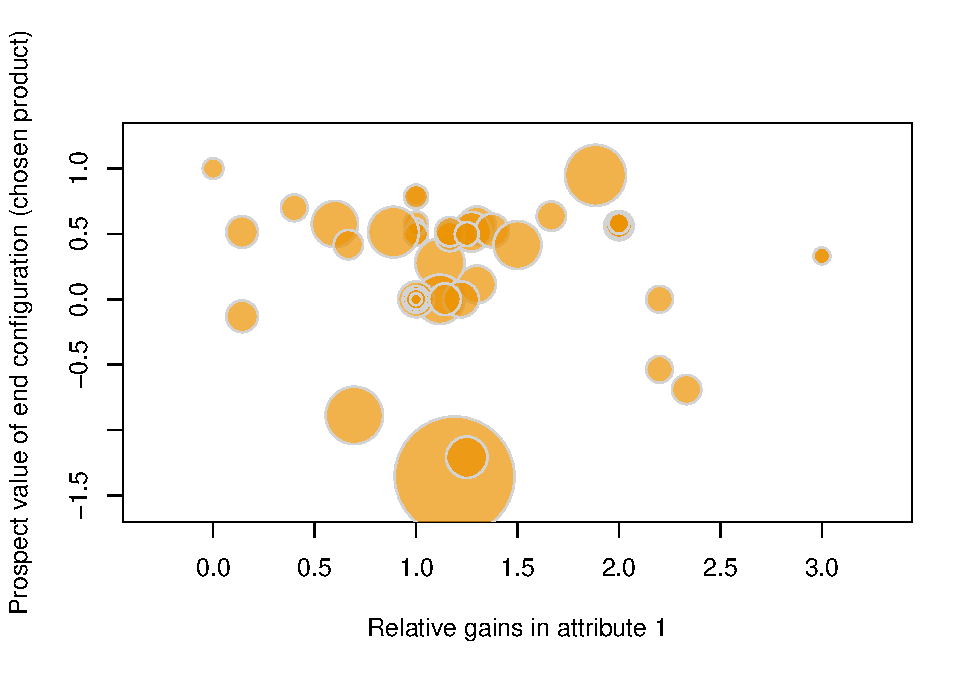
\includegraphics{Test3_files/figure-latex/unnamed-chunk-9-1.pdf}

\end{document}
